%%%  BP: Determine applications affected by upgrade
%%%  Copyright (C) 2014 Jakub Kadlčík, <jakub.kadlcik@upol.cz>
%%%  Tento soubor vychází z dokumentu kidiplom.tex
%%%  https://github.com/martinrotter/kistyles/blob/master/kidiplom.tex


%%%  Ukázkový text a dokumentace stylu pro text závěrečné (bakalářské a
%%%  diplomové) práce na KI PřF UP v Olomouci
%%%  Copyright (C) 2012 Martin Rotter, <rotter.martinos@gmail.com>
%%%  Copyright (C) 2014 Jan Outrata, <jan.outrata@upol.cz>


%%  Pro získání PDF souboru dokumentu je třeba tento zdrojový text v
%%  LaTeXu přeložit (dvakrát) programem pdfLaTeX.

%%  V případě použití programu BibLaTeX pro tvorbu seznamu literatury
%%  je poté ještě třeba spustit program Biber s parametrem jméno
%%  souboru zdrojového textu bez přípony a následně opět (dvakrát)
%%  přeložit zdrojový text programem pdfLaTeX.

%%  Postup získání Postscriptového souboru je popsán v dokumentaci.


%%  Třída dokumentu implementující styl pro závěrečnou práci. Vybrané
%%  nepovinné parametry (ostatní v dokumentaci):

%%  'master' pro sazbu diplomové práce, jinak se sází bakalářská práce

%%  'field=kód' pro Váš studijní obor, kódy pro diplomovou práci 'uvt'
%%  pro Učitelství výpočetní techniky pro střední školy a 'binf' pro
%%  Bioinformatiku, jinak je výchozí Informatika, a pro bakalářskou
%%  práci 'ainfk' pro Aplikovanou informatiku v kombinované formě,
%%  'inf' pro Informatiku, 'infv' pro Informatiku pro vzdělávání a
%%  'binf' pro Bioinfomatiku, jinak je výchozí Aplikovaná informatika
%%  v prezenční formě

%%  'printversion' pro sazbu verze pro tisk (nebarevné logo a odkazy,
%%  odkazy s uvedením adresy za odkazem, ne odkazy do rejstříku),
%%  jinak verze pro prohlížeč

%%  'biblatex' pro zapnutí podpory pro sazbu bibliografie pomocí
%%  BibLaTeXu, jinak je výchozí sazba v prostředí thebibliography

%%  'language=jazyk' pro jazyk práce, jazyky english pro anglický,
%%  slovak pro slovenský, jinak je výchozí czech pro český

%%  'font=sans' pro bezpatkový font (Iwona Light), jinak výchozí
%%  patkový (Latin Modern)

\documentclass[
%  master,
  field=inf,
%  printversion,
  biblatex,
%  language=english,
%  font=sans,
  glossaries,
  index
]{kidiplom}

%% Informace pro úvodní strany. V jazyku práce (pokud není v komentáři
%% uvedeno česky) a anglicky. Uveďte všechny, u kterých není v
%% komentáři uvedeno, že jsou volitelné. Při neuvedení se použijí
%% výchozí texty. Text pro jiný než nastavený jazyk práce (nepovinným
%% parametrem language makra \documentclass, výchozí český) se zadává
%% použitím makra s uvedením jazyka jako nepovinného parametru.

%% Název práce, česky a anglicky. Měl by se vysázet na jeden řádek.
\title{Nalezení aktualizacemi ovlivněných aplikací}
\title[english]{Determine applications affected by upgrade}

%% Volitelný podnázev práce, česky a anglicky. Měl by se vysázet na
%% jeden řádek. Výchozí je prázdný.
\subtitle{}
\subtitle[english]{}

%% Jméno autora práce. Makro nemá nepovinný parametr pro uvedení
%% jazyka.
\author{Jakub Kadlčík}

%% Jméno vedoucího práce (včetně titulů). Makro nemá nepovinný
%% parametr pro uvedení jazyka.
\supervisor{doc. RNDr. Michal Krupka, Ph.D.}

%% Volitelný rok odevzdání práce. Výchozí je aktuální (kalendářní)
%% rok. Makro nemá nepovinný parametr pro uvedení jazyka.
%\yearofsubmit{\the\year}

%% Anotace práce, včetně anglické (obvykle překlad z jazyka
%% práce). Jeden odstavec!
\annotation{Práce se zabývá problematikou \uv{aktualizacemi ovlivněných aplikací}, konkrétně pak jejich nalezením a doporučením nejlepšího způsobu, jak docílit jejich restartování. V teoretické části se zabývá otázkou důležitosti tohoto problému a pojednává o možných algoritmech. Součástí práce je vytvoření nástroje pro vyhledávání ovlivněných aplikací na linuxové distribuci Fedora. Tento nástroj by mělo být možné použít také skrze rozšíření balíčkovacího systému DNF.}

\annotation[english]{This thesis deals with the topic of „applications affected by upgrade“, particularly of their determination and recommending the best way of achieving their restart. In the theoretical part it shows the relevance of the problem and describes possible algorithms. This thesis also includes the tool for determining affected applications on Fedora linux distribution which should be possible to use via an extension of the DNF package manager.}

%% Klíčová slova práce, včetně anglických. Oddělená (obvykle) středníkem.
\keywords{aktualizace systému, ovlivněné aplikace, Python, Fedora, DNF}
\keywords[english]{system updates, affected applications, Python, Fedora, DNF}

%% Volitelná specifikace příloh textu práce, i anglicky. Výchozí je '1
%% CD/DVD'.
%\supplements{jedno kulaté placaté CD/DVD s malou kulatou dírou uprostřed}
%\supplements[english]{one round flat CD/DVD with a small round hole in the middle}

%% Volitelné poděkování. Stručné! Výchozí je prázdné. Makro nemá
%% nepovinný parametr pro uvedení jazyka.
\thanks{Rád bych poděkoval doc. RNDr. Michalu Krupkovi, Ph.D. za cenné rady a pomoc při tvorbě této práce. Děkuji také společnosti Red~Hat,~Inc., jmenovitě pak Ing.~Miroslavu~Suchému, za inspirativní spolupráci.}

%% Cesta k souboru s bibliografií pro její sazbu pomocí BibLaTeXu
%% (zvolenou nepovinným parametrem biblatex makra
%% \documentclass). Použijte pouze při této sazbě, ne při (výchozí)
%% sazbě v prostředí thebibliography.
\bibliography{bibliografie.bib}

%% Další dodatečné styly (balíky) potřebné pro sazbu vlastního textu
%% práce.
\usepackage{lipsum}



%%%
%%%  !! Není v oficiálním stylu !!
%%%
\usepackage{import}
\definecolor{mygreen}{rgb}{0,0.6,0}
\definecolor{mygray}{rgb}{0.5,0.5,0.5}
\definecolor{mymauve}{rgb}{0.58,0,0.82}

\lstdefinestyle{sources}
{%
	backgroundcolor=\color{white},   % Pozadí
	commentstyle=\color{mygreen},    % Komentáře
	keywordstyle=\color{blue},       % Klíčová slova jazyka
	stringstyle=\color{mymauve},     % Řetězce
}

\lstset
{%
	%
	% Základní nastavení
	%
	basicstyle=\footnotesize,        % Styl a typ písma
	captionpos=b,                    % Pozice popisku
	showstringspaces=false,          % Když true, místo mezer se vypíše podtržítko. e.g. "Hello_world"
	title=\lstname,                  % Při výpisu zdrojového kódu ze souboru, nastaví název souboru jako popisek
	tabsize=4,                       % Velikost tabulátoru (počet mezer)
	style=sources,
	%
	% Podpora českých znaků
	% http://tex.stackexchange.com/questions/30512/how-to-insert-code-with-accents-with-listings/85947#85947
	%
	literate=
		{á}{{\'a}}1     {í}{{\'i}}1     {é}{{\'e}}1
		{ý}{{\'y}}1     {ú}{{\'u}}1     {ó}{{\'o}}1
		{ě}{{\v{e}}}1   {š}{{\v{s}}}1   {č}{{\v{c}}}1
		{ř}{{\v{r}}}1   {ž}{{\v{z}}}1   {ď}{{\v{d}}}1
		{ť}{{\v{t}}}1   {ň}{{\v{n}}}1   {ů}{{\r{u}}}1
		{Á}{{\'A}}1     {Í}{{\'I}}1     {É}{{\'E}}1
		{Ý}{{\'Y}}1     {Ú}{{\'U}}1     {Ó}{{\'O}}1
		{Ě}{{\v{E}}}1   {Š}{{\v{S}}}1   {Č}{{\v{C}}}1
		{Ř}{{\v{R}}}1   {Ž}{{\v{Z}}}1   {Ď}{{\v{D}}}1
		{Ť}{{\v{T}}}1   {Ň}{{\v{N}}}1   {Ů}{{\r{U}}}1
	,
}




\begin{document}
%% Sazba úvodních stran -- titulní, s bibliografickými údaji, s
%% anotací a klíčovými slovy, s poděkováním a prohlášením, s obsahem a
%% se seznamy obrázků, tabulek, vět a zdrojových kódů (pokud jejich
%% sazba není vypnutá).
\maketitle

%% Vlastní text závěrečné práce. Pro povinné závěry, před přílohami,
%% použijte prostředí kiconclusions. Povinná je i příloha s obsahem
%% přiloženého CD/DVD.

%% -------------------------------------------------------------------

\newcommand{\BibLaTeX}{\textsc{Bib}\LaTeX}



%%%
%%%  Text práce
%%%

\section{Úvod}
	Ve většině distribucí GNU/Linuxu se software standardně spravuje prostřednictvím balíčkovacího systému. Jedná se o nástroj zajišťující evidenci nainstalovaného a dostupného softwaru, jeho instalaci a následnou aktualizaci. Nové distribuce většinou vznikají odvozením jiné, již existující distribuce a v tomto případě bývá zachován typ balíčků i balíčkovací systém. Můžeme tedy říct, že distribucí je mnoho, ale balíčkovaích systémů se používá jen velmi málo. Konkrétně lze hovořit o distribucích GNU/Linuxu používající balíčky RPM\footnote{RPM = Red Hat Package Manager}, DEB\footnote{DEB = Debian software package} a nebo jiný typ balíčku. V posledním případě se jedná případ od případu o velmi specifický předpis balíčku. V rámci této práce se budeme zabývat linuxovou distribucí Fedora jakožto reprezentantem první skupiny.
	\\
	\\
	Fedora vznikla jako nekomerční odnož Red Hat Linuxu a zachovala stávající systém balíčků RPM\@. Od své první verze využívá nástavbu nad RPM zvanou YUM\@. Ten se po čase stal z mnoha technickůch důvodů nedostatečný a proto se objevila alternativa pojmenovaná DNF\@. V současné době lze paralelně využívat oba tyto nástroje, avšak je snaha YUM kompletně nahradit za pomocí DNF\@.
	\\
	\\
	Když spustíme aplikaci, do paměti se načtou knihovny a soubory potřebné k jejímu běhu. Pokud je některá z knihoven, nebo samotná aplikace po dobu jejího běhu aktualizována, v paměti stále zůstanou původní soubory, přestože fyzicky už nemusí existovat (mohou být smazány, nebo nahrazeny novějšími verzemi).
	\\
	Zjistit, které, v systému spuštěné, aplikace využívají takto neaktuální soubory, není pro uživatele triviální. V současné době sice existují nástroje, které tento problém řeší, avšak jsou z mnoha důvodů nedostatečné.
	\\
	\\
	Na první pohled by se mohlo zdát, že postrádá smysl, zabývat se takovým problémem a jeho vyřešení nepřinese nic zajímavého. Ve skutečnosti však mohou být důsledky velmi nebezpečné. Pokud například aktualizace opravuje bezpečnostní chybu staré verze, běžící aplikace zůstanou neopravené. K jejich opravě dojde až jejich restartováním. Uživateli se tak může stát, že nainstaluje záplatu, bude si myslet, že jeho systém je opět bezpečný a přitom stále běží několik nebezpečných procesů.
	Další problém se týká spíše uživatelů \textit{unstable} distribucí, kterým do systému mohou přicházet zpětně nekompatibilní balíčky. Potom se může stát, že některá služba odmítne nastartovat, protože nová verze nepovoluje stávající konfiguraci, nebo vlivem nepřesně specifikovaných závislostí zůstane v systému nekompatibilní verze knihovny. Takovýchto případů bychom si rádi všimli, co nejdříve to bude možné, nikoliv až v kritické chvíli, kdy například dojde k restartování serveru.
	\\
	\\
	V současné době sice existují nástroje, které tento problém řeší, avšak jsou z mnoha důvodů nedostatečné, viz kapitola \ref{porovnani-s-konkurenci}. Práce si proto klade za cíl vytvořit software, který bude řešit problém \textit{nalezení aktualizacemi ovlivněných aplikací}. Software by měl najít všechny programy využívající neaktuální soubory a doporučit jejich restartování. Pro různé typy programů by měla být vypsána jiná doporučení a nápověda, jakým způsobem to lze provést.

	\section{Požadavky}
	Tato práce vznikala ve spolupráci se společností Red~Hat,~Inc., přičemž následující požadavky byly zhotoveny na základě již existujícího zadání.
	\\
	\\
	Teoretická část práce by se měla zabývat problematikou aktualizacemi ovlivněných aplikací a otázkou jejich vyhledání. Budou uvedeny a vysvětleny algoritmy pro řešení tohoto problému. Výsledkem práce bude software implementující některý z teoreticky popsaných algoritmů.
	\\
	\\
	Software bude implementován v programovacím jazyce Python a jeho cílovou platformou bude linuxová distribuce Fedora, pro kterou bude k dispozici instalační balíček. Vývoj software bude probíhat pod svobodnou licencí splňující kritéria pro přidání balíčku do oficiálních repozitářů této distribuce. Zdrojový kód programu bude umístěný na libovolném veřejném úložišti a bude komukoliv k dispozici.
	\\
	Software by měl disponovat textovým uživatelským rozhraním a mělo by být možné jej používat přímo skrze balíčkovací systém. Z tohoto důvodu bude taktéž popsána problematika tvorby rozšíření pro balíčkovací systém DNF\@.

\section{Analýza problému}
V této kapitole rozebereme problematiku na dílčí části, navrhneme algoritmy pro jejich vyřešení a provedeme úvahu nad vhodností jejich použití. Nejdříve se zaměříme na samotné získání aktualizacemi ovlivněných aplikací, poté zvážíme univerzálnost navrhovaného řešení napříč operačními systémy a nakonec se zaměříme na to, jakým způsobem lze nalezené aplikace restartovat.

	\subsection{Seznam ovlivněných aplikací -- Ilustrativně}
	Hlavním účelem programu bude nalezení aktualizacemi ovlivněných, běžících aplikací. Řešení se zdá být velmi přímočaré. Nejdříve zjistit seznam balíčků, které byly od spuštění systému modifikovány. Následně pro každý balíček zjistit seznam souborů, které poskytuje. Poté zjistit, které procesy využívají některý z množiny modifikovaných souborů. Tedy pro každý spuštěný proces zjistit seznam souborů jež využívá a najít shodu se soubory poskytovanými modifikovanými balíčky.

	\newpage
	\lstinputlisting
	[
		language={Python},
		label=naive-tracer-algorithm,
		caption={Algoritmus pro vypsání seznamu ovlivněných aplikací}
	]{sources/naive_tracer_algorithm.py}

	Algoritmus na první pohled vypadá velmi jednoduše a zřejmě vypíše korektní množinu procesů. Mohlo by se tedy zdát, že máme hotovo, nicméně jsme nevzali v úvahu časovou složitost takového algoritmu. Ta, jak si ukážeme níže, je bohužel velmi nepříznivá, což by vedlo k útrpně pomalému vyhledávání.

		\subsubsection*{Časová složitost}
		Časovou složitost lze vyjádřit následovně. První průchod přes všechny balíky je lineární, tedy $O(n)$. Pro každý balík se prochází všemi procesy, takže násobíme $* O(m)$. Protože jsou obě $m$ i $n$ spočetně velké a nejsou to konstanty, místo $O(n*m)$ vyjádříme $O(n^2)$.
		\\
		\\
		Dále počítáme složitost množinového průniku. V případě jeho naivní implementace, která porovnává každý prvek jedné množiny s každým prvkem druhé, dostaneme kvadratickou složitost $O(n^2)$. V případě optimalizovanějšího návrhu si polepšíme na $O(n)$.
		\\
		\\
		Množinový průnik je zjišťován pro každou kombinaci balíčku a procesu, proto původní $O(n^2)$ násobíme $O(n)$ (případně $O(n^2)$ při naivní implementaci). Výslednou časovou složitost ukázaného algoritmu tedy vyčíslíme jako $O(n^3)$, případně $O(n^4)$.

	\subsection{Seznam ovlivněných aplikací -- Vylepšení}
	\label{seznam-ovlivnenych-aplikaci-vylepseni}
	Klíčem k rychlejšímu získání chtěných procesů je zvolení vhodné vyhledávací struktury pro data. Vezměme si fakt, že mnoho procesů využívá stejné soubory (např. knihovny). Naivní algoritmus tedy jeden konkrétní soubor musí ověřit hned několikrát -- pro každý proces, který jej využívá.

	Tento nedostatek můžeme řešit tak, že nebudeme zkoumat proces po procesu, ale místo toho vezmeme množinu všech souborů v paměti, přičemž ke každému souboru si poznačíme procesy, které jej využívají. Pro nejrychlejší možné vyhledávání v množině souborů, zvolíme strom typu BTree jako strukturu pro uložení dat. Zaplatíme sice zvýšenou spotřebou paměti, ale jak si ukážeme v kapitole XY, rychlostní zlepšení bude na první pohled zjevné.

	\newpage
	\lstinputlisting
	[
		language={Python},
		label=tracer-algorithm,
		caption={Vylepšený algoritmus pro vypsání seznamu ovlivněných aplikací}
	]{sources/tracer_algorithm.py}

		\subsubsection*{Časová složitost}
		Při vyhledávání je pro každý balíček procházen seznam jím poskytovaných souborů. Složitost tohoto problému je analogická předchozí situaci, tedy $O(n^2)$. Co se ovšem změnilo, je problém nalezení všech procesů, využívajících daný soubor. Nyní si stačí vyzvednout jejich seznam jednorázovým přístupem do stromové struktury typu BTree. Složitost tohoto problému je $O(log(n)$. Poskládáním jednotlivých kousků problému dohromady, získáváme časovou složitost celého algoritmu vyjádřenou jako $O(n^2 * log(n))$.

	\subsection{Informace o aplikaci}
	Na chvíli se zamysleme nad přenositelností nástroje mezi různými linuxovými distribucemi. Položme si následující otázku, je možné zjišťovat informace o aplikacích stejným způsobem na libovolném linuxovém systému? Prozradím, že část z nich skutečně ano, avšak ne všechny.

	Rozlišujeme totiž dva druhy informací. Pracujeme se spuštěnými aplikacemi, tedy lze hovořit o procesech spuštěných v systému. Každý proces má nějaký PID\footnote{PID (Process ID) je unikátní atribut pro identifikaci procesu}, spustil jej nějaký uživatel, běží určitou dobu, apod.

	Dále lze uvažovat, že každá\footnote{Každá standardně nainstalovaná} aplikace je poskytována distribučním balíčkem. Každý takový balíček poskytuje informace o tom, k čemu slouží, v jaké je verzi, jak dlouho je nainstalován, apod.

	Lze předpokládat, že informace o procesech budou získatelné jednotným způsobem napříč celým spektrem linuxových distribucí, avšak informace o balíčku budou závislé na jeho typu. Jejich struktura se totiž výrazně liší, používají jiné názvy atributů a tak podobně.

	\subsection{Jak aplikaci restartovat?}
	\label{jak-aplikaci-restartovat}
	Aplikace můžeme rozdělit do několika kategorií. Zřejmě budou existovat takové, jež nemůžeme restartovat jinak, než rebootováním celého operačního systému. Příkladem budiž init, či jaderné procesy. Dále jistě budou v systémech s grafickým uživatelským rozhraním aplikace, k jejichž restartování bude potřeba řestartovat celé grafické prostředí. Příkladem mohou být správci oken a aplikace související s uživatelským sezením\footnote{Známější spíše v anglickém originále jako session}. V těchto případech nezbývá jiná možnost, než provést požadovanou operaci jako reboot počítače, či odhlášení a opětovné přihlášení uživatele do grafického režimu.
	\\
	\\
	Zajímavější situace je v případě aplikací, které lze restartovat pomocí příkazu v příkazové řádce. Ta je typická, nikoliv však výhradní, pro tzv.\ daemony, či služby. Napříč velkým spektrem distribucí a správců služeb, lze k jejich restartování standardně použít příkaz \texttt{service} \textit{název\_služby} \texttt{restart}. Podobně lze tímto způsobem přistupovat i ke spoustě běžných aplikací, u nich se ale budou jednotlivé příkazy fundamentálně lišit.
	\\
	\\
	Všechny ostatní aplikace spadají do poslední skupiny. Uživatel je musí ručně ukončit a znovu spustit. Nezáleží na tom, zda jsou grafické a bude tak učiněno křížkem v záhlaví okna, nebo spuštěné v příkazové řádce a budou ukončeny jiným způsobem. Tato poslední kategorie není bezpečně automatizovatelná a proto musí zůstat v plné režii uživatele.

\section{Linuxová distribuce Fedora}
Fedora je linuxová distribuce GNU/Linuxu vzniklá jako nekomerční odnož Red~Hat Linuxu. Odtud převzala stávající systém balíčků RPM, nad kterým poskytuje nástavby v podobě správců balíčků YUM a novějším DNF. Fedoru vyvíjí komunita vývojářů okolo Fedora Project, sponzorovaného firmou Red Hat. Projekt vznikl v roce 2003, kdy se firma rozhodla rozdělit Red Hat Linux na komerční Red Hat Enterprise Linux a komunitní Fedoru.
\\
\\
Správce balíčků YUM byl nedílnou součástí Fedory již od jejího prvního vydání Fedora Core 1, avšak v aktuálně stabilní verzi Fedora 22 došlo k jeho nahrazení nástrojem DNF. Nyní lze používat oba nástroje paralelně, avšak YUM je označen za zastaralý a v příštím vydání bude ze systému kompletně odstraněn. Důvody nahrazení jdou mimo rámec této práce, nicméně jedním z nich, pro tuto práci významným, je modularita systému DNF.
\\
\\
Projekt se skládá z knihovny hawkey, poskytující aplikační rozhraní pro jazyky C a Python ke knihovně libsolv, samotného nástroje DNF a dále pak sbírkami rozšíření \texttt{dnf-plugins-core} a \texttt{dnf-plugins-extras}, pomocí kterých lze vylepšovat jeho funkcionalitu. Do těchto sbírek lze za určitých podmínek nechat zahrnout i vlastní rozšíření.

\newpage
\section{Programovací jazyk Python}
Jedním z požadavků této práce je, aby výsledný produkt byl realizován v programovacím jazyce Python. Proč je tomu tak a proč zrovna Python? Na tuto otázku existuje velmi jednoduchá odpověď. Nový balíčkovací systém DNF, distribuce Fedora, je napsán právě v tomto jazyce a poskytuje v něm API pro tvorbu rozšíření od třetích stran. Nehledě na to, Python disponuje několika vlastnostmi, ve kterých konkurence zaostává.

	\subsection{Historie}
	Koncept jazyka Python vznikl na konci osmdesátých let dvacátého století v Amsterdamském CWI\footnote{Centrum Wiskunde \& Informatica (English: National Research Institute for Mathematics and Computer Science)}. Jeho autorem je Guido van Rossum, který dosud stále stojí v čele jeho vývoje. Při návrhu Pythonu se inspiroval jazykem ABC, na kterém v té době pracoval. Implementace započala v prosinci 1989 a první stabilní verze 1.0 vyšla o několik let později, v roce 1994. Od té doby se vývoj posunul o dvě major verze dopředu. Řada 2.x.x odstartovala v roce 2000 a je stále velmi populární, obzvláště pak v komerční sféře.  V roce 2008 vyšla verze 3.0, která měla být nástupcem dvojkové řady, avšak kvůli neúplné zpětné kompatibilitě probíhá vývoj obou řad paralelně. Aktuálně lze tedy Python získat ve dvou stabilních verzích. V době psaní této práce se jedná konkrétně o verze 2.7.9 a 3.4.3.

	\subsection{Vlastnosti}
	% @TODO Najít slovo koerce ve slovníku
	Python je platformově nezávislý, multi-paradigmatický programovací jazyk, jehož výchozím stylem je strukturované, případně objektově orientované programování. Poskytuje však mnohé prvky funkcionálního paradigmatu, jako například lambda výrazy, iterátory, ne-destruktivní varianty většiny standardních funkcí, či funkce \texttt{map}, \texttt{filter}, \texttt{apply} a další, dobře známé z ostatních funkcionálních jazyků.
	\\
	\\
	Typování je v tomto jazyce dynamické, avšak silné. Kupříkladu operaci sčítání tedy nelze provést na jednom argumentu typu číslo a druhém argumentu typu řetězec, i kdyby v něm byla uložena číselná hodnota. K žádným koercím a implicitnímu přetypování v tomto případě nedojde a výsledkem operace bude chyba. Velmi výrazným rysem je takzvaný duck typing, který preferuje provedení dané operace s objektem, aniž by se předem ověřoval jeho typ. Při selhání zjevně objekt nebyl požadovaného typu a situace se vyřeší výjimkou. V opačném případě objekt poskytoval požadované rozraní a byl tedy správného typu.
	\\
	\\
	Standardní knihovna se snaží být \uv{rozumně} velká a všechna dodatečná funkcionalita je řešena formou rozšíření. Hlavní implementace Pythonu zvaná CPython je napsaná v jazyce C standardu C89. Tento překladač proramy kompiluje do přechodného bytekódu (soubor s příponou \texttt{.pyc}), který je následně prováděn virtuálním strojem. O správu paměti se stará garbage collector.

	\subsection{Filozofie}
	Rady a doporučení, jak by měl vypadat zdrojový kód v jazyce Python, sepsal Tim Peters v dokumentu PEP 20 -- The Zen of Python. Jak sám píše na začátku dokumentu, principy shrnul do dvaceti aforismů, z nichž však pouze devatenáct bylo zapsáno. Následuje ukázka samotného Zenu:

	\begin{verse}
	Beautiful is better than ugly.\\
	Explicit is better than implicit.\\
	Simple is better than complex.\\
	Complex is better than complicated.\\
	Flat is better than nested.\\
	Sparse is better than dense.\\
	Readability counts.\\
	\end{verse}

	Zbývajících dvanáct veršů naleznete ve zmíněném dokumentu, případně v interpretru jazyka, pomocí příkazu \texttt{import this}.

	\subsection{Syntax a sémantika}
	Základním syntaktickým rysem, kterým se syntax liší od jazyků rodiny C je použití odsazení k vyhrazení bloku kódu, namísto složených závorek. Přídává klíčové slovo \texttt{with}, které umožní otevřít zdroj, implementující metody \texttt{\_\_enter\_\_} a \texttt{\_\_exit\_\_}, pro daný blok kódu. Konstrukt se sám postará o ukončení práce se zdrojem a to i v případě, kdy ve vykonávaném kódu dojde k chybě. V jazyce nenajdeme konstrukci \texttt{switch}. Návrh o její přídání byl oficiálně zamítnut, viz PEP 3103. K dispozici máme několik základních datových struktur jako jsou seznamy (obdoba pole), slovníky (obdoba asociativního pole), tuply, či množiny. Všechny se používají velmi snadno, například seznam lze vytvořit zapsáním jeho prvků mezi hranaté závoky.
	\\
	\\
	Doporučené konvence pro formátování zrojového kódu popisuje dokument PEP 8. Pojednává například o způsobu odsazování, doporučené šírce řádku, komentářích, způsobech pojmenování různých elementů a podobně.


	\subsection{Kompatibilita verzí}

\newpage
\section{Implementace}
Již jsme se seznámili s prostředím linuxových systémů a problematikou hledání aktualizacemi ovlivněných aplikací. Ukázali jsme si také konkrétní vyhledávací algoritmy předpokládající jisté vstupní parametry, jako například seznam modifikovaných balíčků, nebo seznam všech procesů. Samotný algoritmus pak zjišťoval seznam souborů poskytovaných daným balíčkem, či seznam souborů využívaných daným procesem. V této kapitole si vysvětlíme, jakým způsobem lze v jazyce Python zmíněné vstupní parametry získat a také, jakým způsobem realizovat potřebné operace.

	\subsection{Práce s procesy}
	Správu procesů v jazyce Python zajišťuje modul \texttt{psutil}, který je ve Fedoře k dispozici pod názvem \texttt{python-psutil}. Tento modul umožňuje získání seznamu všech aktuálně běžících procesů a poskytuje přístup ke všem jejich atributům, které lze v linuxových systémech zjistit. Mimo to poskytuje rozhraní pro získávání informací o paměti, procesoru, pevných discích a síťových rozhraních.

	Nás ovšem zajímá pouze práce s procesy. Ukázku, jak vypadá rozhraní objektu procesu, vidíme v následujícím příkladu.

	\lstinputlisting
	[
		language={Python},
		label=psutil,
		caption={Základní práce s procesy v psutil}
	]{sources/psutil.py}

	Můžeme požadovat i pokročilejší funkce, jako například zjištění souborů, které daný proces využívá. Pro následující ukázku předpokládejme identifikátor některého z procesů uložený v proměnné \texttt{pid}.

	\lstinputlisting
	[
		language={Python},
		label=process-files,
		caption={Výpis všech souborů, které proces využívá}
	]{sources/process_files.py}

	Výpis tohoto ukázkového kódů může vypadat následovně:

	\lstinputlisting
	[
		label=process-files-output,
		caption={Ukázka výstupu předchozího kódu}
	]{sources/process_files_output}

	Jak jsme mohli vidět, objekty procesů jsou vytvářeny na základě jejich identifikátoru PID\@. Zjištění seznamu jejich hodnot je tedy klíčkovou záležitostí, kterou pro nás zajišťuje funkce \texttt{psutil.get\_pid\_list()}.

	\subsubsection{Problémy při práci s procesy}
		Při práci s procesy narážíme na několik problémů, které bychom neustále měli mít na paměti.
		\\
		\\
		K prvnímu výraznému jevu dochází, když je vytvořen objekt reprezentující proces, poté je daný proces ukončen a následovně dojde k pokusu o přístup k atributu jeho objektu. Obdobná situace nastává v případě získání seznamu identifikátorů všech spuštěných procesů a následného vytvoření objektů na jejich základě. Může se totiž stát, že došlo k ukončení některých procesů mezi časem získání jejich identifikátoru a časem vytváření objektů. V těchto případech dochází k výjimce, se kterou však není potřeba si příliš lámat hlavu. Proces byl již ukončen, takže pro naše účely není ničím zajímavý\footnote{Ukončený proces zjevně aktualizací ovlivněn nebude}. Je však důležité si tuto problematiku uvědomit.
		\\
		\\
		Dále si lze všimnout poměrně zvláštního jevu. Tím jsou podivné řetězce na konci názvů, některých procesem používaných, souborů. Množinu všech možných přípon, které se mohou vyskytnout, nedovedu přesně určit, nicméně v průběhu tohoto projektu jsem se setkal s následujícími případy:

		\lstinputlisting
		[
			language=SQL,
			label=strings-in-filenames,
			caption={Artefakty v názvech souborů}
		]{sources/strings_in_filenames}

		Tyto soubory samozřejmě fyzicky neexistují. Například na konci prvního zmíněného souboru přebývá řetězec \texttt{;53c7cd86}. Po jeho vyjmutí z názvu, však získáme cestu ke skutečně existujícímu souboru poskytovanému balíčkem \texttt{kde-plasma-nm}. Obdobně to platí i pro příponu \texttt{.\#prelink\#} a jí následovaný identifikátor, nebo příponu \texttt{\#new}. Je potřeba si také dát pozor na příznak \texttt{(deleted)}, který se může objevit i nezávisle na těchto příponách.

	\subsection{Práce s balíčky}
		Především nás budou zajímat tři operace. Zjištění seznamu balíčků, které byly od daného času modifikovány, zjištění základních informací o konkrétním balíčku, jako například název, popis, atd. a nakonec zjištění seznamu souborů, které balíček poskytuje. Ukážeme si, že každou z nich lze implementovat několika různými způsoby. Objasníme, který z nich vyhovuje potřebám této práce nejvíce a proč tomu tak je.

		\subsubsection{Databáze balíčků}
		Úvodem uděláme drobnou odbočku a podíváme se, jakým způsobem jsou v systému reprezentovány informace o balíčcích.
		\\
		\\
		Balíčkovacím systémem distribuce Fedora je program zvaný DNF\@, který pro uchovávání historie operací, prováděných s balíčky, využívá sqlite databázi v adresáři \texttt{/var/lib/dnf/history}. Z ní se můžeme dozvědět informace o všech proběhlých transakcích. Schéma databáze vypadá následovně.

		\centerline{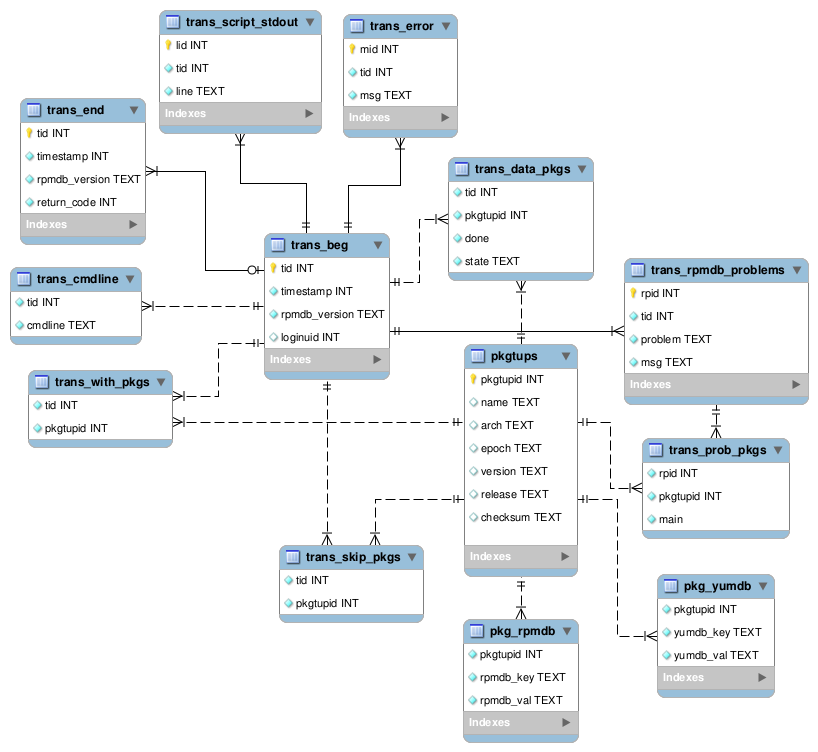
\includegraphics[scale=0.45]{images/dnf-database.png}}

		My se budeme zajímat výhradně o úspěšně proběhlé transakce, proto nás tabulky, zabývající se chybovýmy stavy, nebudou zajímat. Nám užitečné informace se nacházejí především v tabulkách \texttt{trans\_beg}, \texttt{trans\_end}, \texttt{trans\_data\_pkgs} a \texttt{pkgtups}. Z prvních dvou lze zjistit, kdy byly proběhlé transakce spuštěny a dokončeny. Kterých balíčků se týkali a jaké operace s nimi byly prováděny, popisuje tabulka \texttt{trans\_data\_pkgs}. Dané balíčky ovšem rozlišuje pouze pomocí jejich unikátního identifikátoru \texttt{pkgtupid}. Pro zjištění více informací o daném balíčku je nutné nalézt jeho záznam v poslední zmíněné tabulce \texttt{pkgtups}.

		\subsubsection{Historie balíčků}
		Na základě znalostí z předchozí kapitoly můžeme bez dalších odboček přejít přímo ke zkoumání historie balíčků. V programovacím jazyce Python máme pro práci se sqlite databázemi k dispozici balíček \texttt{sqlite3}. Ten umožní dotazování se vůči databázi pomocí vlastních SQL dotazů. Nejdříve se tedy zaměříme na vytvoření dotazu pro získání všech balíčků modifikovaných od určitého bodu v čase.
		\\
		\\
		Informace o balíčcích, jako například jeho název, nebo verze, jsou uloženy v tabulce \texttt{pkgtups}. Není zde však datum jeho změny, proto musíme začít z druhého konce. Provedené transakce včetně času jejich spuštění se nacházejí v tabulce \texttt{trans\_beg}. Odtud dovedeme transakce spojit s relacemi v tabulce \texttt{trans\_data\_pkgs} přes atribut \texttt{tid}. Výsledkem spojení budou relace obsahující atribut \texttt{pkgtupid}, pomocí jenž můžeme provést spojení s tabulkou \texttt{pkgtups}, o kterou nám z počátku šlo.
		\\
		Současným mezivýsledkem jsou všechny relace vzniklé spojením zmíněných tabulek. Pomocí restrikce tuto relaci omezíme pouze na relace pro které platí, že atribut \texttt{trans\_beg.timestamp} nabývá hodnot větších než $t$, kde $t$ je argument ve formátu definovaném jako Unix time\footnote{Známém také jako POSIX time, nebo Epoch time. Tento formát popisuje počet sekund uplynulých od 00:00:00 světového času dne 1.~1.~1970}.

		V jazyce SQL lze tento problém vyjádřit následovně.

		\lstinputlisting
		[
			language=SQL,
			label=packages-newer-than-sql,
			caption={Balíčky změněné od času $t$ - SQL dotaz}
		]{sources/packages_newer_than.sql}

		Pokračujme spuštěním tohoto dotazu v jazyce Python a získáním jeho výsledku. Předpokládejme předchozí dotaz\footnote{Nutno nahradit proměnnou $t$ symbolem otazníku} uložený v proměnné \texttt{sql}, umístění databázového souboru v proměnné \texttt{db\_file} a libovolný čas uvedeného formátu v proměnné \texttt{unix\_time}. Tento zdrojový kód ukazuje, jak se lze dotázat vůči dané sqlite databázi a získat výsledek.

		\lstinputlisting
		[
			language=Python,
			label=packages-newer-than-py,
			caption={Balíčky změněné od času $t$ - Python}
		]{sources/packages_newer_than.py}

		Ukázkový kód je natolik sebevysvětlující, že se obejde bez většího komentáře. Za pozornost stojí především metoda \texttt{fetchall()}, která vrací seznam všech záznamů výsledku. Ve výchozím nastavení jsou jednotlivé záznamy reprezentovány datovou strukturou \texttt{tuple}. Jedná se o strukturu, která by se dala nejlépe popsat jako uspořádaná n-tice. Při přístupu k hodnotám atributů potom záleží na jejich pořadí v n-tici. Tento přístup má velké nevýhody, proto na třetím řádku ukázkového kódu specifikujeme, že chceme jednotlivé záznamy vracet reprezentované pomocí objektů třídy \texttt{sqlite3.Row}. To umožní přístup k atributům pomocí jejich názvů.

		\subsubsection{Informace o balíčku}
		V předchozí kapitole jsme pracovali s databázovým souborem, uchovávajícím informace o proběhlých operacích s balíčky. Odtud jsme dokázali zjistit například jejich název, verzi a pár dalších. Nicméně o balíčcích lze zjišťovat informací mnohem více. Jsou však uloženy na jiném místě\footnote{V databázi RPMDB umístěné v adresáři \texttt{/var/lib/rpm/}} a proto musíme k problému přistupovat novým způsobem.
		\\
		Pro zjištění všech, o balíčku dostupných informací, můžeme použít příkaz:

		% Pozor, balíček musí být nainstalován
		\begin{lstlisting}
			rpm -qi nazev_balicku
		\end{lstlisting}

		Výpis těch zajímavějších můžeme vidět zde:
		\lstinputlisting
		[
			label=fedora-package-info-output,
			caption={Informace o balíčku}
		]{sources/fedora_package_info_output}

		Tyto informace lze v prostředí jazyka Python získat a zpracovat v zásadě dvěma způsoby. Prvním je použití modulu \texttt{subprocess} ke spuštění výše zmíněného příkazu a získání jeho výstupu.
		\lstinputlisting
		[
			language=Python,
			label=fedora-package-info-parse,
			caption={Parsování informací o balíčku}
		]{sources/fedora_package_info_parse.py}

		Tato varianta však není ideální. Vyžaduje ruční parsování výstupu, jakožto textového řetězce. Navíc dochází k drobnému zpomalení z důvodu spouštění nového procesu. Tato prodleva by byla zanedbatelná v případě jednorázového volání. Informace však mohou být zjišťovány o velkém množství balíčků, což by vedlo k výraznému zpomalení programu.

		Mnohem lepší variantou je použití aplikačního rozhraní, poskytovaného modulem \texttt{rpm}, které nabídne čistější řešení, netrpící zmíněnými neduhy.

		\lstinputlisting
		[
			language=Python,
			label=fedora-package-info-api,
			caption={Získání informací o balíčku pomocí rpm API}
		]{sources/fedora_package_info_api.py}

		V tomto kódu se vyskytuje spousta neobjasněných elementů. Pojďme si je postupně projít a vysvětlit jejich význam. Každý skript pracující s balíčkem RPM musí zákonitě začínat instancováním třídy \texttt{TransactionSet}. Ta se postará o otevření databáze balíčků a poskytne rozhraní pro dotazování se vůči ní. Tím je metoda \texttt{dbMatch} použitá na následujícím řádku. Jejím výsledkem je vždy iterátor obsahující nalezené balíčky. To, jaké balíčky budou hledány, lze ovlivnit nastavením patřičných argumentů. V případě jejich vynechání, bude vrácen iterátor množiny všech nainstalovaných balíčků. Samozřejmě lze i vyhledávat pouze balíčky splňující určitá kritéria. V ukázkovém příkladu jsou vyhledány všechny balíčky, které se jmenují \texttt{vim-X11}. Jméno balíčku je však unikátní vlastnost, takže iterátor obsahuje pouze jednu položku (případně žádnou pokud nebyla nalezena shoda). Získáme ji pomocí metody \texttt{next()}.
		\\
		Jednotlivé balíčky jsou reprezentovány pomocí slovníků\footnote{Jiný název pro konstrukci známější především jako asociativní pole}. To znamená, že jejich klíči jsou textové řetězce \texttt{"name"}, \texttt{"summary"}, \texttt{"group"} a tak podobně. Konstanty \texttt{RPMTAG\_SUMMARY}, \texttt{RPMTAG\_GROUP}, apod. slouží pouze jako tenká abstrakční vrstva, vracející daný řetězec.

		\subsubsection{Seznam souborů poskytovaných balíčkem}
		Každý balíček v sobě nese množinu souborů, které při instalaci nakopíruje do systému. Říkejme, že balíček tyto soubory poskytuje. V případě, že dva balíčky poskytují tentýž soubor, jsou navzájem vyloučeny. To znamená, že není možné, nainstalovat je současně. O každém souboru v operačním systému lze tedy říci, že v daný moment, je poskytován nanejvýš jedním balíčkem\footnote{Nikoli však právě jedním, protože, ne každý soubor v systému musí být vlastněn nějakým balíčkem. Protipříkladem budiž uživatelská data}.
		\\
		\\
		Pro zjištění seznamu všech souborů poskytovaných daným balíčkem, slouží příkaz:

		% Pozor, balíček musí být nainstalován
		\begin{lstlisting}
			rpm -ql nazev_balicku
		\end{lstlisting}

		K získání a zpracování tohoto seznamu platí totéž, co v předchozím případě. Varianta využívající modul \texttt{subprocess}, by vypadala velmi podobně. Oproti předchozímu použití, by se změnil pouze spouštěný příkaz. Navíc jsme tuto variantu implementace z dobrých důvodů vyloučili, proto se budeme zabývat především použitím aplikačního rozhraní modulu \texttt{rpm}.

		\lstinputlisting
		[
			language=Python,
			label=fedora-package-files-api,
			caption={Získání seznamu souborů poskytovaných balíčkem}
		]{sources/fedora_package_files_api.py}

		V tomto ukázkovém příkladu nově narážíme na funkci \texttt{fi} její výsledky. Tato funkce pro daný balíček vrací objekt reprezentující seznam, jím poskytovaných souborů včetně jejich atributů. Položkami tohoto seznamu jsou uspořádané n-tice, jejichž první složku tvoří název souboru.

	\subsection{Vyhledání ovlivněných aplikací}
	V předchozích kapitolách jsme si vysvětlili, jak v programovacím jazyce Python získat všechny data, které algoritmus popsaný v kapitole \ref{seznam-ovlivnenych-aplikaci-vylepseni} na svém vstupu vyžaduje. Nyní bychom se mohli podívat na konkrétní implementaci tohoto algoritmu. Nicméně, neučiníme tak, protože samotná implementace není ničím zajímavá. Jedná se pouze o přepis pseudokódu z téže kapitoly do zdrojového kódu jazyka Python. Z tohoto důvodu bych případné zájemce rád odkázal přímo na zdrojový kód programu.

	\newpage
	\subsection{Rozšíření pro balíčkovací systém DNF}
	DNF poskytuje aplikační rozhraní pro tvorbu dvou druhů rozšíření. Prvním z nich je takzvaný plugin, jenž může implementovat metody, které budou provedeny v daných momentech instalačního procesu. Spustit vlastní kód tedy lze například během čtení konfiguračních souborů, před provedením plánované transakce, či ihned po ní. Vykonat lze libovolný kód, nicméně zajímavá je především možnost zkoumat prováděnou transakci a operace s balíčky, jež se chystá provést. Nemusí se však jednat pouze o čtení. Transakci lze podle vlastních potřeb libovolně upravovat. Druhý typ rozšíření umožňuje tvorbu vlastních příkazů, které lze spustit v příkazové řádce skrze program \texttt{dnf}.
	\\
	\\
	Implementace vlastního příkazu potom může vypadat následovně.

	\lstinputlisting
	[
		language=Python,
		label=dnf-command,
		caption={Ukázka vlastního příkazu pro program \texttt{dnf}}
	]{sources/dnf_command.py}

	Při spuštění, ukázkový příkaz pouze vypíše, jakým způsobem byl zavolán. Pro zprovoznění je nutné soubor uložit do adresáře definovaného v konfiguračním souboru jako \texttt{pluginpath}. Ve výchozím nastavení se jedná o adresář \texttt{/usr/lib/python2.7/site-packages/dnf-plugins/}. A dále zaregistrováním příkazu do uživatelského rozhraní, které můžeme zajistit pomocí následujícího pluginu.

	\lstinputlisting
	[
		language=Python,
		label=dnf-command-register,
		caption={Plugin registrující vlastní příkaz}
	]{sources/dnf_command_register.py}

	Nyní, podíváme-li se pomocí \texttt{dnf help} do nápovědy, vidíme příkaz \texttt{foo}, který jsme vytvořili naším rozšířením. Zavoláme jej jednoduše pomocí \texttt{dnf foo arg1 arg2 arg3}.

	Na závěr této vsuvkové kapitoly si ještě ukážeme plugin, který za každou úspěšně provedenou transakcí vypíše seznam balíčků, jež nainstalovala.

	\lstinputlisting
	[
		language=Python,
		label=dnf-plugin,
		caption={Plugin vypisující seznam transakcí nainstalovaných balíčků}
	]{sources/dnf_plugin.py}



\newpage
\section{Tracer}
	V předchozích kapitolách jsme představili problematiku hledání aktualizacemi ovlivněných aplikací, popsali algoritmy pro jejich hledání a způsob, jak je lze implementovat v jazyce python pro linuxovou distribuci Fedora. Nyní se podíváme na projekt nesoucí název Tracer, jenž na těchto základech vznikl.
	\subsection{Uživatelská příručka}
		Následuje pouze nástin možných případů užití. Kompletní manuálovou stránku programu naleznete v příloze \ref{manualova-stranka-programu-tracer}.

		\subsubsection{Standardní použití}
		\label{standardni-pouziti}
		Primárním a zároveň nejjednodušším způsobem, jak program spustit, je příkazem\footnote{Oprávnění superuživatele je nutné, protože program potřebuje číst databázi balíčkovacího systému.} \texttt{sudo tracer}. Na výstupu obdržíme seznam ovlivněných aplikací, tak jak byl požadován v zadání. Ukázkový výstup můžeme vidět na následujícím příkladu.

		\lstinputlisting
		[
			label=tracer-standard-usage-output,
			caption={Ukázkový výstup příkazu \texttt{sudo tracer}}
		]{sources/tracer_standard_usage_output}

		Formát výstupu je koncipován především z pohledu uživatelské přívětivosti, proto jsou nalezené aplikace jsou rozděleny dle kategorií popsaných v kapitole \ref{jak-aplikaci-restartovat}. První skupinu aplikací lze restartovat pouhým zkopírováním bloku navrhovaných příkazů do terminálu.
		\\
		\\
		Ve výchozím stavu se vypíše pouze poznámka o nerestartovatelných aplikacích, namísto celého jejich seznamu, protože s nimi uživatel stejně nemůže nic udělat. Z obnobného důvodu jsou vypsány pouze aplikace současného uživatele. Pro vypsání všech aplikací všech uživatelů, lze použít přepínače \texttt{-{}-all} a \texttt{-{}-everyone}.

		\pagebreak
		\subsubsection{Zobrazení konkrétní aplikace}
		Uživatel může ve výstupu narazit na aplikaci, kterou například nezná, nebo netuší, proč je potřeba ji restartovat a jak toho docílit. Z tohoto důvodu existuje přepínač \texttt{-s} neboli \texttt{-{}-show}, jenž zobrazí všechny informace, které Tracer o aplikaci zná a se kterými pracuje.

		\lstinputlisting
		[
			label=tracer-helper-output,
			caption={Ukázkový výstup příkazu \texttt{sudo tracer -s apache2}}
		]{sources/tracer_helper_output}

		Stejně jako u většiny UNIXových programů, lze množství vypisovaných informací ovlivnit přepínači \texttt{-v} a \texttt{-vv}. První varianta zobrazí i seznam balíčků, jenž aplikaci ovlivnil. Druhá varianta pak zobrazí i seznam konkrétních souborů, které balíčky aktualizovali a aplikace je využívá. Konečně, výpis těchto pomocných informací ke každé nalezené aplikaci, lze spustit přepínačem \texttt{-{}-helpers}.

		\subsubsection{Interaktivní mód}
		V určitých případech může uživatel chtít zobrazit pomocné informace pouze k několika aplikacím, ale nechce vypisovat jejich názvy. Pro tento účel byl zaveden interaktivní režim. Pokud spustíme Tracer s parametrem \texttt{-i}, nebo \texttt{-{}-interactive}, obdržíme na výstupu očíslovaný seznam aplikací zakončený promptem. Postupně zadáváme čísla aplikací, které nás zajímají a dostáváme výpis pomocných informací.

		\subsubsection{DNF plugin}
		Specialitou program pro uživatele linuxové distribuce Fedora je rozšíření pro balíčkovací systém DNF, spouštějící program Tracer po každé úspěšně provedené transakci. Tedy je spuštěno automaticky po nainstalování, aktualizaci, či odstranění libovolného balíčku. Toto rozšíření nevyžaduje žádnou interakci s uživatelem a není potřeba jej nijak manuálně nastavovat. Výstup vypadá totožně s ukázkou v kapitole \ref{standardni-pouziti}.

	\subsection{Licence}
	Program je vyvíjen pod svobodnou licencí GNU/GPLv2, jejíž plné znění naleznete v příloze \ref{gnu-gpl-v2}. Tato licence zajišťuje, že každý člověk má právo studovat zdrojový kód tohoto programu. To znamená číst jej, modifikovat a libovolně s ním experimentovat. Původní, nebo pozměněné dílo může dále distribuovat, avšak pod podmínkou, že tyto klony budou poskytovat stejná práva, jako původní software. Licence navíc umožňuje využívat dílo k libovolnému účelu.
	\\
	\\
	Při použití této licence můžeme o Traceru hovořit jako o otevřeném, či ještě lépe, svobodném software.

	\subsection{Verzování}
	Přirozeným požadavkem na software, je \uv{rozumný} způsob jeho verzování. Na první pohled to sice nemusí být zřejmé, ale případní uživatelé musejí být schopni určit, jakou verzi používají. A to hned z několika důvodů. Software se v průběhu času vyvíjí a uživatelé by jej měli průběžně aktualizovat\footnote{To je ostatně motivací této práce}. K tomu je ovšem potřeba identifikovat používanou verzi a dokázat určit, zda je jiná verze novější, nebo ne. Programátoři navíc nejsou neomylní a jejich dílo může obsahovat chyby. V případě jejich hlášení je nutné uvést verzi programu, která danou chybou trpí, jinak bude velmi problematické, až nemožné, ji nalézt a opravit.
	\\
	\\
	Z tohoto důvodu Tracer k verzování využívá nástroje GIT, kde je každá logická\footnote{Určitá posloupnost změn tvořící pojmenovatelný celek, týkající se právě jednoho tématu} úprava zdrojového kódu uložena jako popis transformačních kroků, potřebných pro převedení stávajícího kódu na nový. Krokům k provedení jedné logické změny se v kontextu nástroje GIT říká commit. Každý takový commit je označen pomocí kontrolního součtu a dle historie commitů lze určit jejich pořadí. Určité milníky potom lze označit a přiřadit jim vlastní název (tag). Tím například může být číslo verze.
	\\
	\\
	Člověk využívající vývojovou větev Traceru může tedy identifikovat přesnou verzi pomocí kontrolního součtu nejnovějšího commitu, případně pomocí jména tagu.


	\subsection{Zdrojový kód}
	Jakožto svobodný software, má Tracer zdrojové kódy a vše co k nim patří, veřejně vystavené. Kdokoli tak může uplatnit práva zaručená licencí GNU/GPLv2. Pro vytvoření vlastní kopie zdrojového kódu ve svém počítači, spusťte příkaz:

	\begin{lstlisting}[gobble=12]
		git clone https://github.com/FrostyX/tracer.git
	\end{lstlisting}

	Takto bude získána nejaktuálnější verze zdrojového kódu, která neprošla řádným testovacím procesem a v žádném případě ji nelze považovat za stabilní. Její užití je doporučeno pouze vývojářům programu Tracer a lidem majícím zájem o pohled na novou funkcionalitu tohoto programu. Avšak pouze na vlastní nebezpečí.

	\subsection{Instalační balíčky pro Fedoru}
	Cílovou platformou tohoto programu je linuxová distribuce Fedora. Zde je jeho zprovoznění velmi přímočaré. Nainstalovat lze buď pouze samotný program Tracer, jež bude potřeba manuálně spouštět, nebo i plugin pro balíčkovací systém DNF\@, který jej bude spouštět automaticky. Jsou distribuovány odděleně. Samotnou instalaci lze provést pomocí balíčkovacích systémů YUM, DNF, či jejich grafických nadstaveb. Následující ukázka vysvětlí instalaci skrze balíčkovací systém DNF.

	\lstinputlisting
	[
		language=Sh,
		label=dnf-install-tracer,
		caption={Instalace programu Tracer pomocí balíčkovacího systému DNF}
	]{sources/dnf_install_tracer.sh}

	Tyto příkazy zajistí stažení a instalaci balíčků, včetně všech potřebných závislostí. Získány budou z oficiálního repozitáře distribuce Fedora, pravděpodobně tedy nebude nainstalována stejná verze programu, jako ta, která je přibalená na CD této práce.
	\\
	\\
	Přibalenou verzi lze nainstalovat spuštěním následujícího příkazu:

	\lstinputlisting
	[
		language=Sh,
		label=rpm-install-tracer,
		caption={Instalace přiložené verze programu Tracer}
	]{sources/rpm_install_tracer.sh}

	\subsection{Dokumentace}
	Původní dokumentace projektu byla kolekce souborů oddělená od zdrojového kódu programu a uživatelům byla poskytována prostřednictvím wiki systému. Nevýhodu tohoto řešení jsem si uvědomil záhy po jeho nasazení. Ve chvíli, kdy je dokumentace oddělena od zdrojového kódu, nastává problém s rozlišováním, pro kterou verzi kódu je určena. Jde-li o vydanou stabilní verzi, lze ji samozřejmě specifikovat někde v textu. Nicméně v případě vývojové větvě lze těžko určit, od kterého commitu popisovaná funkcionalita funguje.
	\\
	\\
	Mnohem lepším řešením je vedení dokumentace přímo v adresáři zdrojového kódu programu. O oboje se pak stará stejný verzovací systém a tím pádem je k dispozici dokumentace věrně odpovídající zdrojovému kódu v libovolném okamžiku. Projekt nyní využívá nástroj sphinx, který na základě souborů ve formátu rst\footnote{reStructuredText -- plaintextový formát umožňující intiutivní strukturování dokumentu} dokáže vygenerovat dokumentaci v několika výstupních formátech, jako například HTML, či PDF. Do jednotlivých stránek navíc umožňuje vkládat konkrétní entity zdrojového kódu. Odkaz na webovou dokumentaci projektu naleznete v kapitole \ref{odkazy}. Vlastní verzi si můžete vygenerovat pomocí příkazů:

	\lstinputlisting
	[
		language=Sh,
		label=rpm-generate-docs,
		caption={Vygenerování dokumentace pomocí nástroje sphinx}
	]{sources/generate_docs.sh}

	\subsection{Lokalizace}
	Přestože projekt obsahuje velmi jednoduché uživatelské rozhraní a nejspíš jej lze používat i s elementárními znalostmi angličtiny, poskytuje možnost jazykových lokalizací. Součástí zdrojových kódů je soubor \texttt{tracer.pot} obsahující všechny lokalizovatelné řetězce a dalé pak soubory s příponou \texttt{.po}, obsahující překlady těchto řetězců do konkrétních jazyků. Tyto soubory jsou vyvěšeny na překladatelském serveru \url{http://transifex.com}.
	\\
	\\
	Při vytváření instalačního balíčku se ze všech \texttt{.po} souborů vygenerují jejich binární verze s příponou \texttt{.mo}. Ty jsou při instalaci balíčku kopírovány do systémového adresáře s překlady. V závislosti na uživatelem preferovaném jazyku systému, je při spuštění vybrána kýžená lokalizace. V současné době existuje kompletní překlad pouze do českého jazyka, přičemž ostatním uživatelům bude zobrazena výchozí anglická verze.

	\subsection{Programátorská příručka}
	Tato kapitola je určená především novým vývojářům a všem zájemcům, kteří chtějí nějakým způsobem pracovat se zdrojovými kódy projektu. Objasní jejich organizaci, použitá paradigmata a poradí, jak ověřit, že jimi provedené změny neměly nezamýšlený, nežádoucí efekt.

		\subsubsection{Architektura zdrojového kódu}
		V domovském adresáři projektu najdeme pouze soubory potřebné k balíčkování a konfigurační soubory pro služby jež projekt využívá. Dále vidíme několik adresářů, z nichž zajímavé jsou především tyto následující. Spouštěcí soubor programu nalezneme v adresáři \texttt{bin}. Tento soubor obsahuje pouze nejnutnější minimum zdrojového kódu, nutného k zavedení programu. Naopak naprostá většina kódu se nachází v adresáři \texttt{tracer}, který je při instalaci nakopírován k systémovým modulům jazyka Python.
		\\
		\\
		Tento kód je povětšinou objektově orientovaný a koncepčně je rozdělen do jednotlivých celků architektury Model-View-Controller (MVC). Šablony (View), nejsou tvořeny pomocí speciálního šablonovacího systému, jako tomu často bývá například u webových aplikací, nýbrž jde o obyčejné soubory obsahující zdrojový kód jazyka Python. Slouží však pouze k vypsání výstupu na požadované zařízení. Kontrolery se starají o naplnění těchto šablon \uv{vypočítanými} daty. Největším celkem jsou modely tvořící zbytek adresáře. Ty slouží ke zjišťování informací o systému, procesech, balíčcích, zajišťují se o jazykovou lokalizaci a jiné.

		\subsubsection{Testování}
		Zdrojový kód projektu je prověřován pomocí jednotkových testů, i testů uživatelského rozhraní. Oboje jsou realizovány pomocí modulu \texttt{unittest}. Testy však nepokrývají každou jednotlivou řádku kódu a negarantují stoprocentní spolehlivost, nicméně za určitých okolností, například při refaktorování, jsou velmi nápomocné. Navíc jsou pomocí CI spouštěny automaticky při uložení libovolné změny do verzovacího systému. Ručně, v příkazové řádce, lze testy spustit například pomocí nástrojů \texttt{nosetests}, nebo \texttt{unit2}.

	\subsection{Odkazy}
	\label{odkazy}
	V tuto chvíli bych rád uvedl přehledovou tabulku s odkazy na všechny důležité služby, které projekt využívá.

	\begin{table}[h]
		\begin{tabular}{ll}
			Homepage:               & \url{http://tracer-package.com/} \\
			Dokumentace:            & \url{http://docs.tracer-package.com/en/latest/} \\
			Zdrojový kód:           & \url{https://github.com/FrostyX/tracer} \\
			Travis CI:              & \url{https://travis-ci.org/FrostyX/tracer} \\
			Transifex (lokalizace): & \url{https://www.transifex.com/organization/frostyx/dashboard/tracer}
		\end{tabular}
	\end{table}


\section{Srovnání s konkurencí}
	\label{porovnani-s-konkurenci}
	Rád bych se pokusil objektivně porovnat svou práci s konkurenčními projekty. Během počátečního průzkumu, než jsem se vůbec začal touto problematikou zabývat, hledal jsem již existující projekt, který bych mohl podpořit, či na něj navázat. Ovšem nenašel jsem jediný a tak vznikl Tracer. V průběhu jeho vývoje jsem postupně narazil na čtyři různé existující nástroje, z nichž některé tu byly již dříve a některé vznikly teprve nedávno.
	\\
	\\
	Nyní si jeden po druhém projdeme, zaměříme se na jejich cíle, vlastnosti, podporované operační systémy, uživatelské rozhraní a podobně.
	\subsection{needs-restarting}
	% - potřebuje roota
	% - vypisuje duplicitní aplikace (různé pid)
	% - pouze pro yum
	% - deprecated
	% - o hodně pomalejší než tracer?
	% - zabalíčkováno v yum-utils v Date:   Wed Nov 4 12:44:20 2009 -0500 viz:
	% git://yum.baseurl.org/yum-utils.git commit 43e630fb134e78fc44651c203e3fad364acf1b64

	\subsection{checkrestart}
	% - debian only
	% - nejmíń user friendly
	% - v balíčku debian-goodies
	% - vyžaduje roota

	\subsection{needrestart}
	% Homepage: https://fiasko-nw.net/~thomas/tag/needrestart.html
	% Date:   Fri Mar 29 00:12:15 2013 +0100 viz
	% https://github.com/liske/needrestart.git commit 68891433e1e525087cbe57b7e0854cbc9c83afc5
	% - kontroluje jenom daemony
	% + hooky pro dpkg, rpm, pacman
	% - perl
	% - není ve fedoře
	% + kontejnery
	% + interpretery
	% + lze vyhledat starý kernel
	% + nepotřebuje roota
	% + rychlý
	% - původně určený pouze k vyhledání serviců (změna ve 2.0)

	\subsection{Shrnutí}
	% - nejhorší UI má checkrestart
	% - checkrestart vypadává kvůli debian-only
	% - doposud se ve fedoře primárně používal needs-restarting
	% - needsrestarting je obsolete kvuli yumu
	% - moje snaha o jeho nahrazení pomocí traceru
	% - needrestart se zdá být hodně dobrý
	% - needsrestart vznikl současně s tracerem a funkcionalitou si konkurují
	% - needsrestart ale není zabalíčkovaný
	% - nelze určit nejlepší nástroj, hodně bude záležet na osobních preferencích každého uživatele


\newpage
\section{Život projektu}
% @TODO Přesunout před srovnání s konkurencí?
Projekt tracer spatřil světlo světa v říjnu roku 2013. Už v této době poskytoval většinu současné funkcionality, avšak se v průběhu let výrazně vyvinul. Doposud vyšlo 21 verzí, přičemž nejnovější nese označení 0.6.1. Když vývoj započal, používala se Fedora 19 a jazyk Python byl masivně rozšířený ve verzi 2.7. Nyní jsme se posunuli k Fedoře 22, která je poslední, jež používá tuto verzi Pythonu jako výchozí. Tracer se musel přizpůsobit a nyní je připraven běžet ve Fedoře 23 na Pythonu 3.x. Přiští Fedoru také čeká další významná změna, kterou je nahrazení původního balíčkovacího systému YUM novým nástrojem DNF. Tracer původně fungoval výhradně s YUMem, avšak jak DNF začal získávat na důležitosti, projekt začal podporovat oba systémy současně, aniž by se o to musel uživatel zajímat. Nové verze však od podpory YUMu ze zjevných důvodů upustí.
\\
\\
Zajímavé je také ohlédnutí na způsob distribuce tohoto programu. Od svého počátku byl projekt umístěn na veřejném repozitáři na GitHubu a uživatelé si mohli zdrojové kódy několika způsoby stáhnout. Tento způsob byl vhodný pouze zpočátku, protože uživatelé samořejmě nechtějí instalovat a spravovat závislosti manuálně. V brzké době se proto přešlo na distribuci pomocí vlastního repozitáře v systému COPR. Tato varianta přetrvala dodnes, avšak slouží pouze k vytváření testovacích balíčků. Stabilní verze jsou distribuovány skrze oficiální softwarové repozitáře distribuce Fedora. Autor této práce se stal \uv{balíčkářem} distribuce a o balíček nástroje tracer se stará osobně. Plugin pro systém DNF se podařilo připojit k oficiálně podporovaným komunitním pluginům a jeho distribuci zajišťuje správce této sbírky.
\\
\\
Od samotného počátku nebyla očekávána velká uživatelská základna. Mnoho lidí vůbec netuší, že nástroj tohoto typu vůbec potřebuje a nezajímá je to. Navíc projekt cílí především na uživatele RPM distribucí, protože ostatní již podobný nástroj mají. Počet instalací, potažmo současný počet uživatelů nelze přesně určit. Na základě jistého problému\footnote{\url{https://bugzilla.redhat.com/show\_bug.cgi?id=1187763}} postihujícího všechny uživatele Traceru na Fedoře 21, však lze alespoň určit spodní hranici, již tvoří 240 uživatelů, kteří problém ohlásili. Takovou uživatelskou základnu považuji za úspěch. V rámci zpětné vazby od uživatelů bylo nahlášeno celkem 46 chyb a žádostí o rozšíření funkcionality, z nichž 36 bylo již vyřešeno. Dále bylo vyhověno jedné žádosti o portaci na jinou distribuci.



%% Závěry práce. V jazyce práce a anglicky. Text pro jiný než
%% nastavený jazyk práce (nepovinným parametrem language makra
%% \documentclass, výchozí český) se zadává použitím makra s uvedením
%% jazyka jako nepovinného parametru.
\begin{kiconclusions}
	Cílem mé práce bylo rozebrat problematiku \uv{aktualizacemi ovlivněných aplikací}, konkrétně pak jejich nalezení a doporučení nejlepšího způsobu, jak docílit jejich restartování. V teoretické části jsem objasnil důležitost tohoto problému a důsledky z něho plynoucí. Pokud by si čtenář z tohoto textu odnesl pouze jedinou informaci, měla by to být právě tato. Přestože svůj systém aktualizuje, neznamená to, že se změny automaticky projeví v právě spuštěných aplikacích. Je potřeba je restartovat. Dále jsem zkoumanou problematiku rozdělil na dílčí celky a navrhl algoritmy pro jejich řešení.
	\\
	\\
	Součástí práce bylo v jazyce Python implementovat software pro vyhledávání ovlivněných aplikací na linuxové distribuci Fedora. Zde jsem využil vyzkoumané algoritmy zmíněné výše. V této části bylo zajímavé především získání dat potřebných pro jejich vstupy. Čtenář se dozvěděl, jakým způsobem zjišťovat informace o spuštěných procesech, nainstalovaných balíčcích, či balíčkovacím systémem provedených transakcích.
	\\
	\\
	Původní cílovou platformou byla distribuce Fedora 19 obsahující interpret Pythonu verze 2.7 a balíčkovací systém YUM. V průběhu práce se všechny tyto komponenty staly neaktuálními a proto se projekt přizpůsobil současnému stavu věcí. Fedora je nyní v téměř finální fázi přechodu na systém DNF, v tuto chvíli je již YUM označen za zastaralý a v příštím vydání bude zahozen úplně. Obdobně je tomu v situaci interpreterů Pythonu. Již v příštím vydání bude výchozí jeho třetí verze namísto druhé. Můj projekt tento vývoj reflektuje a je možné jej používat, jak s komponentami, pro které byl určen původně, tak s těmi aktuálními.
	\\
	\\
	Poslední částí mé práce bylo objasnit, jakým způsobem lze rozšiřovat funkcionalitu balíčkovacího systému DNF. Tu považuji za nejméně důležitou, protože pouze rekapituluje již známé a popsané informace. Z tohoto důvodu jí byla věnována pouze jedna kapitola shrnující množinu elementárních znalostí nutných k porozumění zbytku práce.
	\\
	\\
	Software se v průběhu času neustále vyvíjí a vždy jej lze vylepšovat a rozšiřovat o novou funkcionalitu. V případě programu Tracer by například šlo využít nástroje PackageKit, který by mohl přinést podporu pro většinu linuxových distribucí. Má snaha bude nadále směřovat také k zahrnutí programu do výchozí instalace distribuce Fedora, aby si problematiku probíranou v této práci, začalo uvědomovat více uživatelů.
\end{kiconclusions}

\begin{kiconclusions}[english]
	The goal of my thesis was to analyze the topic of „applications affected by upgrade“, particularly of their determination and suggesting the best way of achieving thier restart. In the theoretical part I explained the relevance of this topic and it‘s consequences. If the reader is supposed to learn at least one information from this thesis, it should be this one. Even though he updates his system the changes will not take effect in running applications. It is needed to restart them. Hereafter I divided given topic to sub-units and suggested algorithms for solving them.
	\\
	\\
Part of my work was to implement the software for determining affected applications on linux distribution Fedora, in Python language. Here I utilized algorithms mentioned above. In this part it was mainly interesting to get the data needed on their inputs. The reader learned how to gain information about running processes, installed packages or transactions made by package manager.
	\\
	\\
The initial targeted platform was distribution Fedora 19 with interpreter Python in version 2.7 and package manager YUM installed. During the thesis all of these components became outdated and therefore the project adapted for recent state of things. Fedora is now at final phase of conversion to the DNF manager. At this moment, YUM has been marked as outdated and in the following release it will be removed completely. The Python interpreter is in similar situation. In the following release it‘s third version will be set as default instead of the second version. My project reflects this development and it is possible to use it with the components which it was originally designed for and even with the current components.
	\\
	\\
The last part of my work was to clarify how it is possible to extend the functionality of the DNF package manager. That I consider to be the least important thing because it just sums up already known and described information. Therefore only one chapter was dedicated to wrap up the set of elementary knowledge needed for understanding the rest of the thesis.
	\\
	\\
Software changes constantly and it is always possible to improve it and extend it with new functionality. In case of Tracer program it should be possible to use the PackageKit tool which could bring the support for the most of linux distributions. I will make my effort to have the program included in the default installation of Fedora distribution in order to make more people aware of the topic described in this thesis.
\end{kiconclusions}




%% Přílohy obsahu textu práce, za makrem \appendix.
\appendix

\section{Manuálová stránka programu Tracer}
\label{manualova-stranka-programu-tracer}
\import{appendix/}{manpage.tex}

\newpage
\section{Licence GNU/GPLv2}
\label{gnu-gpl-v2}
\import{appendix/}{gpl-2.0}

%% Obsah přiloženého CD/DVD. Poslední příloha. Upravte podle vlastní
%% práce!
\newpage
\section{Obsah přiloženého CD/DVD} \label{sec:ObsahCD}

\begin{description}

\item[\texttt{doc/}] \hfill \\
  Text práce ve formátu PDF, vytvořený s~použitím závazného stylu KI
  PřF UP v~Olomouci pro závěrečné práce, včetně všech příloh,
  a~všechny soubory potřebné pro bezproblémové vygenerování PDF
  dokumentu textu (v~ZIP archivu), tj.~zdrojový text textu, vložené
  obrázky, apod.

\item[\texttt{src/}] \hfill \\
  Kompletní zdrojové texty programu \textsc{Program} / webové aplikace
  \textsc{Webovka} se všemi potřebnými (příp.~převzatými) zdrojovými
  texty, knihovnami a~dalšími soubory potřebnými pro bezproblémové
  vytvoření spustitelných verzí programu / adresářové struktury pro
  zkopírování na webový server.

\end{description}

%% -------------------------------------------------------------------

%% Sazba volitelného seznamu zkratek, za přílohami.
%\printglossary

%% Sazba povinné bibliografie, za přílohami (případně i za seznamem
%% zkratek). Při použití BibLaTeXu použijte makro
%% \printbibliography. jinak prostředí thebibliography. Ne obojí!

%% Sazba i v textu necitovaných zdrojů, při použití
%% BibLaTeXu. Volitelné.
\nocite{*}
%% Vlastní sazba bibliografie při použití BibLaTeXu.
\printbibliography

%% Bibliografie, včetně sazby, při nepoužití BibLaTeXu.
% \begin{thebibliography}{9}
%\bibitem{kniha2} \uppercase{Hawke}, Paul. NanoHttpd: Light-weight HTTP server designed for embedding in other applications. GitHub [online]. 2014-05-12. [cit. 2014-12-06]. Dostupné z: \url{https://github.com/NanoHttpd/nanohttpd}
%
%\bibitem{jeske13} \uppercase{Jeske}, David; \uppercase{Novák}, Josef. Simple HTTP Server in \csharp: Threaded synchronous HTTP Server abstract class, to respond to HTTP requests. CodeProject: For those who code [online]. 2014-05-24. [cit. 2014-12-06]. Dostupné z: \url{http://www.codeproject.com/Articles/137979/Simple-HTTP-Server-in-C}
%
%\bibitem{uzis2012} \uppercase{ÚSTAV ZDRAVOTNICKÝCH INFORMACÍ A STATISTIKY ČR}. Lékaři, zubní lékaři a farmaceuti 2012 [online]. Praha 2, Palackého náměstí 4: Ústav zdravotnických informací a statistiky ČR, 2012 [cit. 2014-12-06]. ISBN 978-80-7472-089-5. Dostupné z: \url{http://www.uzis.cz/publikace/lekari-zubni-lekari-farmaceuti-2012}
% \end{thebibliography}

%% Sazba volitelného rejstříku, za bibliografií.
\printindex

\end{document}
